\chapter{Sanskrit declension}

Nominal inflection or declension in Sanskrit is of greater varieties than in Pāli, due to the fact that there are more word endings to be considered, including a number of consonants. Unlike the tool of Pāli declension, in which nominal paradigms are implicit and invisible to the users, in Sanskrit we have to treat paradigms explicitly. So, we have two related tools here: \emph{Nominal Paradigms} and \emph{Declension Table}.

\section{Nominal Paradigms}

Generally speaking, a paradigm used for nominal inflection are a typical pattern that can be used for similar nominal words (nouns, pronouns, adjectives) in declension. However, in the program, a paradigm can be an exclusive use for only a single word or just a handful. That is to say, no matter how regular or irregular the declension will be, we call the way of rendition a paradigm.\footnote{The main source of the data is Roderick Bucknell's \emph{Sanskrit Manual}}

The window of paradigm table can be opened by menu Sanskrit > {\faSix \symbol{"F5BF}} Nominal Paradigms. In the first open, you will see all paradigms known to the program listed in the table, with the following information:

\begin{compactenum}
\item Name of the paradigm, usually identical to the nominative singular declension of the sample word (mostly after Bucknell's Manual), if not belonging a special group
\item Gender of the outcome, i.e., Mas, Fem, and Neu, or a combination of these
\item Reference to Bucknell's Manual, for example, \emph{6-2} means Table 6, sub-number 2 (the second paradigm)
\item Nominative Samples, i.e., nominative singular, dual, and plural of the declension
\item Type, i.e., Noun (adjectives included), Pronoun, and Numeral
\end{compactenum}

When a row of paradigm is clicked, the full table of its declension if shown at the bottom. On the right, all terms from the renditions are listed, ordered by endings. You can search for a specific ending by entering some characters. Figure \ref{fig:sanskrit-nomparad} shows what I have described so far, with all terms ending with \pali{e}.

\begin{figure}[!hbt]
\centering
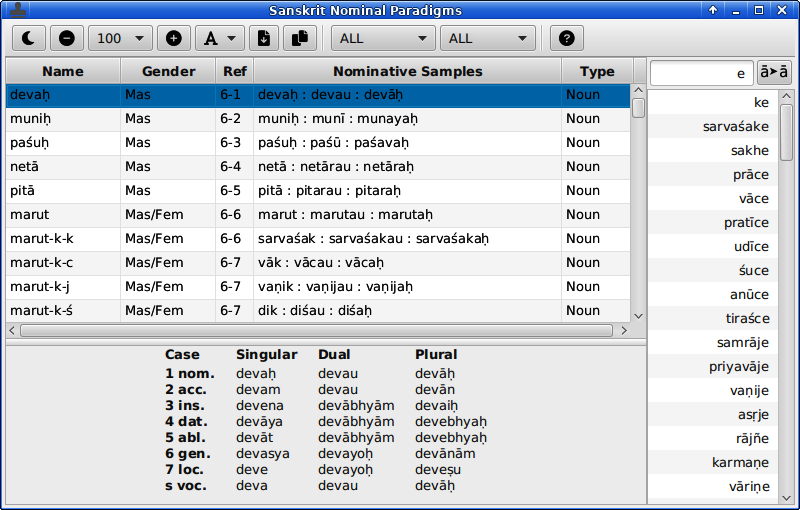
\includegraphics[width=0.9\linewidth]{images/sanskrit-nomparad.png}\\
\caption{Window of Nominal Paradigms}
\label{fig:sanskrit-nomparad}
\end{figure}

\newpage
\boxnote{Paradigms of \pali{marut} and \pali{jagat}\\
\hspace{5mm}There are a number of words ending with certain consonants, (1) as masculine/feminine, grouped by \pali{marut} and \pali{vaṇik}, and (2) as neuter, grouped by \pali{jagat} and \pali{asṛk}.\footnote{The differences between two groups in both genders are in the last character of nominative singular and the last syllable of nominative plural. They are the same in the first group, but different in the second. For masculine/feminine, see Bucknell's Table 6-6, 6-7, and explanations on pp.~19--21. For neuter, see Table 6-21, 6-22, and explanations on p.~23.}\\
\hspace{5mm}The program expands all these cases for each ending, then regroups them under \pali{marut-x-y} and \pali{jagat-x-y} respectively. In the names, \emph{x} is the ending of nominative singular, and \emph{y} is the character used in the last syllable of nominative plural.\\
\hspace{5mm}By this way of arrangement, \pali{vaṇik} and \pali{asṛk} have no name of their own. We have instead \pali{marut-k-j} for \pali{vaṇik}, and \pali{jagat-k-j} for \pali{asṛk}, as well as some others. (Please explore the table carefully by looking at the rendition of sample words.)
}

\section{Declension Table}

The paradigm table shows only known paradigms illustrated by their sample words. We can see applications of these para\-digms upon words in Declension Table.\footnote{The lists of words are taken from the Monier-Williams dictionary.} So, we can see declension of any words, if they can be classified, in this tool. Declension Table can be opened by context menu when you right-click a paradigm in the paradigm table described above. To direct open the tool, use menu Sanskrit > {\faSix \symbol{"F00A}} Declension Table. Figure \ref{fig:sanskrit-decltable} shows the table in the first open.

\begin{figure}[!hbt]
\centering
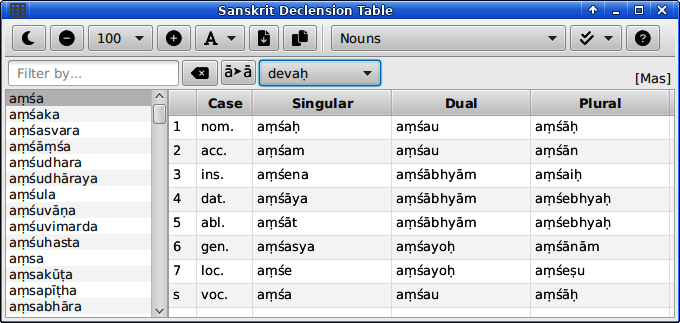
\includegraphics[width=0.9\linewidth]{images/sanskrit-decltable.png}\\
\caption{Window of Declension Table}
\label{fig:sanskrit-decltable}
\end{figure}

At first, you will see nouns in various groups. When you select a word on the left, its declension will be shown in the table. Above the table, there is the paradigm selector. To see words in other paradigms, you have to select your target paradigm.\footnote{Unlike in Pāli, which we can classify normal words by their ending, in Sanskrit grouping of words in each paradigm cannot be done in fully automatic manner. Words in some paradigms have to be added manually. That is why we cannot show you a grand list of words and give you the relevant paradigm when you select a word. We can do at best by selecting a paradigm first and then the relevant words are shown accordingly.} Note that paradigms with only one word in the list are supposed to be irregular. But be aware that in some paradigms giving a full list of words is really difficult, even if those words are supposed to be numerous. This will be the case notably in \pali{marut} and \pali{jagat} groups.

You can switch to other word groups by the selector in the top tool bar. Figure \ref{fig:sanskrit-declpron} shows declension of pronouns and demonstratives. Unlike nouns, which their gender is determined by paradigm, gender of pronouns and demonstratives can be selected by radio buttons above the table.

\begin{figure}[!hbt]
\centering
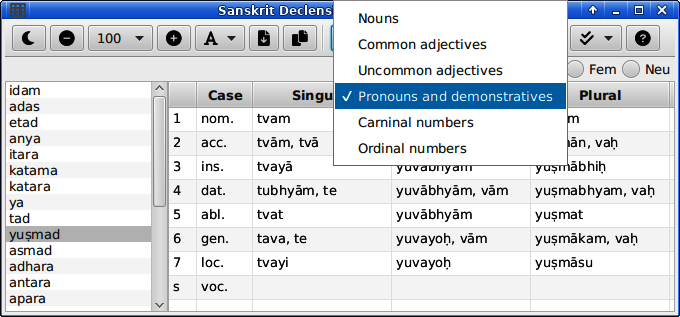
\includegraphics[width=0.9\linewidth]{images/sanskrit-declpron.png}\\
\caption{Declension of pronouns and demonstratives}
\label{fig:sanskrit-declpron}
\end{figure}

Rendering declension of adjectives is a little complicated because they must be declined into three genders. There are two lists of adjectives: (1) common adjectives, ending with \pali{a}, and (2) the uncommon, the rest of those. In the first list, we have to pay attention to feminine rendition of adjectives (see the box note below).

\newpage
\boxnote{Common feminine adjectives\\
When an adjective whose citation form ends with \pali{a} is declined as feminine, there can be either of three results:\\
\hspace{5mm} (1) ending with \pali{ā}\\
\hspace{5mm} (2) ending with \pali{ikā}\\
\hspace{5mm} (3) ending with \pali{ī}
}

So, in common adjectives there are three subgroups, i.e., \pali{ā, ikā,} and \pali{ī}. Except \pali{ā}, the subgroup's marker is shown in parentheses in the list. You have an option to see all of them or one of each group. The selector is above the table. Figure \ref{fig:sanskrit-declcomadj} shows all common adjectives with a feminine declension.

\begin{figure}[!hbt]
\centering
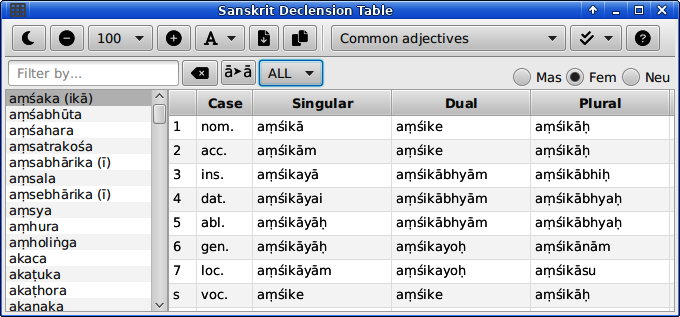
\includegraphics[width=0.9\linewidth]{images/sanskrit-declcomadj.png}\\
\caption{Declension of common adjectives}
\label{fig:sanskrit-declcomadj}
\end{figure}

\newpage
Adjectives having citation form other than \pali{-a} are put together in the uncommon. Here, the selector once used for feminine alternatives now is used for ending selection. There is no difficulty in use here. You just have to know some basic ideas of declension.

Numerals have two word kinds, cardinals and ordinals. Unlike Pāli declension of numbers, which you can compute any number up to six digits, Sanskrit numbers are predefined. You have a fixed list to select. Some numbers have alternative renditions, which can be selected by the drop-down above. Figure \ref{fig:sanskrit-declcard} shows an alternative of 19 selected. Ordinal numbers have similar treatments, so the use is the same. 

\begin{figure}[!hbt]
\centering
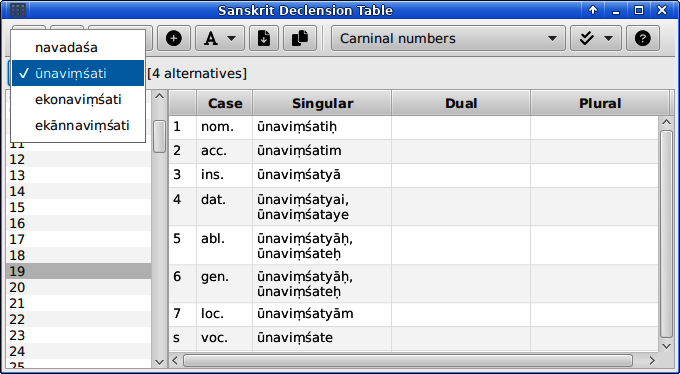
\includegraphics[width=0.9\linewidth]{images/sanskrit-declcard.png}\\
\caption{Alternatives in cardinal numbers}
\label{fig:sanskrit-declcard}
\end{figure}

If you need results in Devanāgarī, you can enable this by the option menu button. Figure \ref{fig:sanskrit-decldeva} shows a result rendered in Devanāgarī.

\newpage
\begin{figure}[!hbt]
\centering
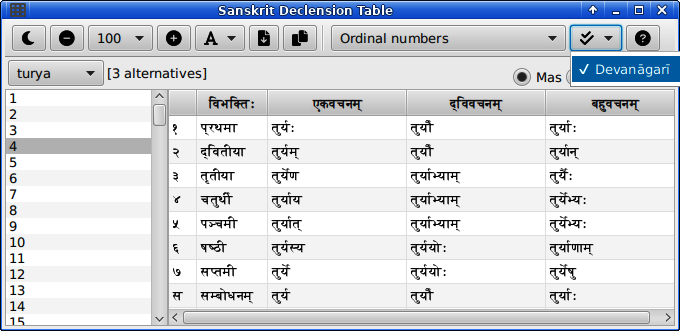
\includegraphics[width=0.9\linewidth]{images/sanskrit-decldeva.png}\\
\caption{Ordinal four rendered in Devanāgarī}
\label{fig:sanskrit-decldeva}
\end{figure}

